\section{\label{II_1_C}Mise en application}

\subsection{Spécificités du corpus traité}
Au sein du chapitre suivant, nous mettrons à l’épreuve l’adaptabilité de l’outil que nous avons décrit pour la segmentation des vidéos en \gls{sequence}s, au corpus d'\gls{Archivesaudiovisuelles} géré au sein du logiciel de Skinsoft. Ce corpus est composé d'archives issues des années 1910 à 1920 essentiellement documentaires, construit par des plans fixes, en noir et blanc et muets. Nous tenterons d’appliquer le processus de segmentation proposé par \gls{pyscene} ur un tel corpus, afin d’en comprendre les données qui pourraient être générées. Le corpus, utilisé ici comme cas d'étude, se caractérise notamment par son ancienneté, et donc par la dégradation de la pellicule sur laquelle l’image s’inscrit. L'outil pourrait ainsi rencontrer des difficultés lors de l’identification des coupures et des changements de plans, brouillés par la dégradation de l’image. Toutefois, la structure du contenu de ces archives facilite la tâche de l’outil, composé d’une succession de \gls{plan}s fixes, dont les coupures sont suffisamment marquées, en fait un corpus relativement bien adapté à ce type de tâche automatique, qui pourrait identifier les coupes plus facilement.  

Par ailleurs, \gls{pyscene}, nous l’avons vu, est un outil dédié à la détection de coupures et à la segmentation d’un flux vidéo en différents plans. Or, dans cette étude, nous cherchons à montrer comment segmenter un flux audiovisuel en différentes séquences, unités sémantiques autonomes. Dès lors, comment paramétrer un tel outil pour la détection d'éléments sémantiques plus larges tels que les \gls{sequence}s ?  

\subsubsection{Paramètres appliqués}

Une solution envisagée serait d'augmenter la valeur du seuil de coupures (treshold), pour que l'outil ne détecte plus les micro-coupures entre les images mais des coupes plus larges, à l'échelle de séquences \footcite{zotero-item-708}. L'outil enregistrerait alors un changement de séquence seulement lors d'une rupture significative de l’espace-temps à l'image. Ce paramétrage reste toutefois limité puisque plusieurs plans adjacents peuvent être radicalement différents d’un point de vue syntaxique, tout en appartenant bien à la même \gls{sequence}. Par exemple, une même \gls{sequence} peut contenir un gros plan et un plan d'ensemble, dont la composition visuelle est bien différente. Dans le cas du corpus d'\gls{Archivesaudiovisuelles} décrit, les plans restent larges et fixes, montrant l'ensemble du décor dans lequel ils s'inscrivent. Ainsi, le paramétrage du seuil pourrait être adéquatement réglé pour la détection de changements de décor, sur ce corpus donné, afin de segmenter le flux vidéo en différentes \gls{sequence}s.  

Par ailleurs, il est possible de régler l’outil sur une durée minimale de détection de coupures à l’aide du paramètre \textit{"min-scene-len"}, pour que le processus n’effectue de coupures qu’après un laps de temps défini \footcite{zotero-item-708}. La définition de ce paramètre nécessite une analyse statistique du corpus segmenté afin d’en définir la durée moyenne d'une séquence. Au sein du logiciel de gestion des collections prévu par Skinsoft, l’institution qui gère ce corpus d’archives documente déjà les séquences contenues par les différentes œuvres au sein des notices de films physiques, sous la forme de repères temporels. Une analyse statistique comparative pourrait être réalisée sur ces données documentées de \textit{time-codes} afin de déterminer la durée moyenne d'une séquence au sein du corpus. D'après nos observations, les séquences extraites sont généralement d'une durée de 60 secondes.

Enfin, sur ce corpus, le mode de détection adaptatif pourrait être privilégié, couplé à une analyse d'images plus importante, permettant à l’outil de comparer le contenu visuel d’un plan par rapport à une grande variété de plans qui l’entourent \footcite{zotero-item-708}. Ce paramètre permettrait encore de régler l’outil sur la détection de changements majeurs dans l'image, dans l'optique d'en extraire uniquement les \gls{sequence}s.  

\subsubsection{Données produites}
Une fois ces paramètres définis, le processus une fois enclenché produit deux types de données en sortie. D'une part, un fichier JSON ou CSV contenant les \textit{time-codes} de début et de fin correspondant aux séquences identifiées au sein de chaque fichier vidéo ingesté. Chaque \gls{sequence} est alors associée à un identifiant unique et à des \textit{times-codes} de début et de fin. D'autre part, l'outil permet également d'extraire pour chaque \gls{sequence} un fichier image, qui correspond à l'image fixe médiane, censée être la plus représentative de la séquence, désignée par le terme d'image clé \footcite{zotero-item-708}. 

Ainsi, la mise en application de l'outil \gls{pyscene}, de l'analyse des données d'origine jusqu'à la production des données de sortie, pourrait être schématisée de la manière suivante (\cref{figpyscene})


\begin{figure}[h!] 
	
	\centering 
	
	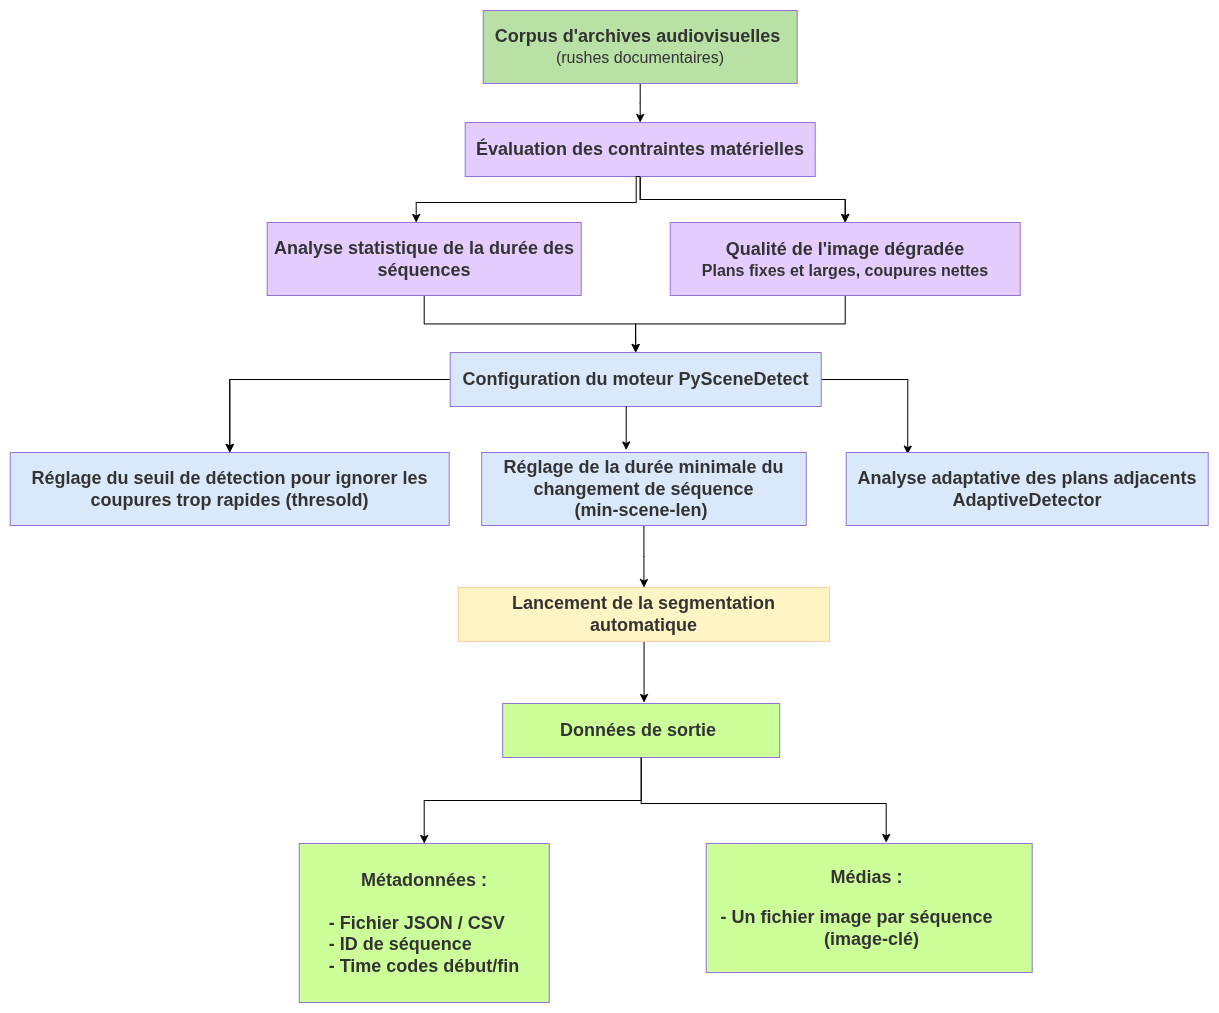
\includegraphics[width=1.0\textwidth]{images/pyscene.png} 
	
	\caption{Mise en application de \gls{pyscene}} 
	
	\label{figpyscene} 
	
\end{figure} 

Toutefois, si ce paramétrage permettrait une plus grande flexibilité pour la segmentation d’un flux vidéo en \gls{sequence}s, l’outil reste limité dans l’automatisation de cette tâche. D’une part l’outil est prévu pour la détection automatique de changement de plan, et d’autre part, une \gls{sequence} ne se définit pas seulement comme une caractéristique syntaxique du langage cinématographique, comme c'est le cas du plan, mais bien par une double caractéristique syntaxique et sémantique. En effet, un changement de séquence concrétise un choix narratif, matérialisé généralement par un changement d’espace-temps. C'est pourquoi, un outil dont l’automatisation est fondée sur des seuils mathématiques reste limité pour une telle tâche. Nous proposons alors de réaliser une analyse sémantique des \gls{sequence}s détectées, afin de ré-associer leur sens à ces coupures détectées automatiquement, tout en réutilisant les données produites : les \textit{times-codes} et l'image clé associés à chaque \gls{sequence}.  